\documentclass{article}

\usepackage{geometry}
\geometry{
	a4paper,
	total={170mm,257mm},
	left=20mm,
	top=20mm,
}

\usepackage[utf8]{inputenc} % allow utf-8 input
\usepackage[T1]{fontenc}    % use 8-bit T1 fonts
\usepackage[hidelinks]{hyperref}       % hyperlinks
\usepackage{url}            % simple URL typesetting
\usepackage{tikz}
\usepackage{dsfont}
\usepackage{amsmath}
\usepackage{array}
\usepackage{float}
\usepackage{rotating}
\bibliographystyle{vancouver}

\title{Supplementary appendix to: \\ {\Large Adjusted age-specific case fatality ratio during the COVID-19 epidemic in Hubei, China, January and February 2020}}


\begin{document}
	
	\maketitle
	
	\section{Introduction}
	
	We model the dynamics of the COVID-19 epidemic in Hubei by date of disease onset from 1 January 2020 to 11 February 2020. 
	In a first step, we use an age-stratified susceptible-exposed-infected-removed (SEIR) compartmental model to describe the dynamics of transmission of the virus in the population of Hubei, including the decrease in incidence after the introduction of control measures on 20 January.
	In a second step, we estimate the mortality of infected individuals with regards to the probability of dying upon infection and the delay between symptom onset and death. 
	We fit the model to data on the time dynamics and the age distribution of both reported cases and deaths.
	We implemented the model in a Bayesian framework using Stan. 
	All code and data are available from \underline{\smash{\url{https://github.com/jriou/covid_adjusted_cfr/}}}.
	
	\section{Data}
	
	
	\begin{table}[h]
		\centering
		\caption{Summary of data sources and fixed parameters.}
		\begin{tabular}{cp{7cm}lll}
			\hline
			Symbol & Comment & Value & Unit & Source \\
			\hline 
			$\mathds{A}$ & Confirmed cases of COVID-19 in Hubei from 1 January to 11 February 2020  & see Fig \ref{fig:data}A & - & \cite{Team2020} \\
			$\mathds{B}$ & Age distribution of all confirmed cases in China up to 11 February 2020 (85\% of these are in Hubei, we assume the age distribution is the same in overall China) & see Fig \ref{fig:data}C & - & \cite{Team2020} \\
			$\mathds{C}$ & Deaths among patients with confirmed COVID-19 infection by day of report in China from 1 January to 11 February 2020 (95\% of these are in Hubei, so the numbers were scaled down by 5\%) & see Fig \ref{fig:data}A & - & \cite{Team2020} \\
			$\mathds{D}$ & Age distribution of the deaths among patients with confirmed COVID-19 infection that occurred in China up to 11 February 2020 (we assume the age distribution is the same in overall China) & see Fig \ref{fig:data}C & - & \cite{Team2020} \\
			$\mathds{E}$ & Age distribution of the population in China & see Fig \ref{fig:data}C & - & \cite{Worldometers.info} \\
			$\mathds{F}$ & $9\times 9$ matrix with contacts between each age class in Shanghai &  see Fig\ref{fig:data}D & per day & \cite{Zhang2019} \\  
			$\mathds{G}$ & Distribution of time from disease onset to death & $\text{log-}\mathcal{N}(20.2,11.6)$ & days & \cite{Linton2020a} \\
			$1/\tau$ & Incubation period & 5.95 & days &  \cite{Bi2020} \\
%			$\psi$ & Proportion of symptomatics & $\text{Beta}(71,18)$ & - & \cite{Bi2020} \\
			$1/\mu$ & Time from disease onset to isolation & 2.4 & days & \cite{Bi2020} \\
			\hline 
		\end{tabular} 
	\end{table}
	
	\begin{figure}[H]
		\centering
		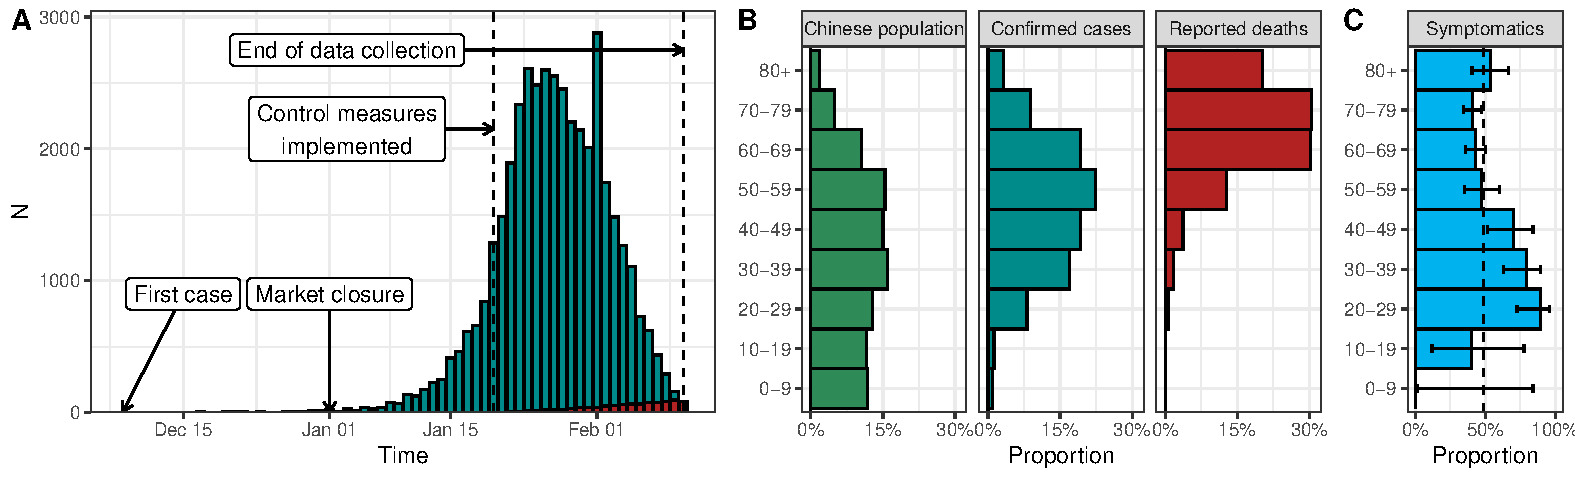
\includegraphics[width=.9\linewidth]{../figures/fig_desc.pdf}
		\caption{Data used to fit the model. (A) Reported confirmed cases of COVID-19 in Hubei by date of disease onset (blue) and reported deaths (red) from 8 December, 2019 until 11 February, 2020 (time point b). Strict control measures were implemented at time point a (23 January). (B) Age distribution of the Chinese population compared to that of confirmed cases of and deaths due to COVID-19. (C) Proportion of individuals infected by COVID-19 showing symptoms among passengers of the Diamond Princess ship (with 95\% credible interval).}
		\label{fig:data}
	\end{figure}
	
	\newpage
	
	\section{Model}
	
	\subsection{Transmission model structure}
	
	We use an age-stratified susceptible-exposed-infected-removed (SEIR) compartmental model using ordinary differential equations (ODEs), with a distinction between asymptomatic and symptomatic infections. 
	We stratify the population in nine ten-year age groups ($0-9, 10-19, \ldots, 70-79, 80+$). 
	The population of each age group $k$ is divided into five compartments: susceptible ($S_k$), incubating or exposed ($E_k$), infected with symptoms ($I_k$), infected and asymptomatic ($A_k$), and removed ($R_k$).
	Note that the number of individuals in each compartment is scaled by the total population of the Hubei province (59,020,000), so that the sum of all compartments is 1.
	Susceptible individuals may become infected through contact with infected individuals with symptoms (assuming that both incubating and asymptomatic individuals are not infectious) from any other age group.
	The force of infection $\lambda_k$ depends on the added number of infectious individuals in each age class, weighted by a contact matrix $\mathds{F}$ and the proportion of infection upon contact with an infectious individual $\beta$.
	
	In addition, we include a time-dependent forcing function to account for the reduction in transmissibility following the introduction of control measures in Hubei on 20 January 2020.
	We use the following logistic function:
	\begin{equation}
	f(t,\eta,\nu, \xi) = \eta + \frac{1-\eta}{1+\exp(\xi *(t-t_1-\nu))}
	\end{equation}
	where $\eta$ is the relative reduction in transmission after control measures are fully implemented, $\xi$ is the slope of the logistic function modelling the implementation of the control measures, and $\nu$ is the delay (in days after 23 January 2020) until the control measures are 50\% effective.
	
	The force of infection $\lambda_k$ can then be expressed as:
	\begin{equation}
	\lambda_k(t) = f(t,\eta,\nu, \xi) \beta S_k(t) \sum_{l=1}^9  \dfrac{I_l(t)}{\mathds{E}_l}  \mathds{F}_{k,l} 
	\end{equation}
	
	\begin{figure}[H]
		\centering
		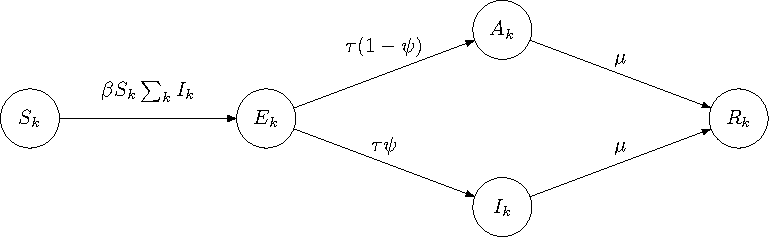
\includegraphics[width=.7\linewidth]{../figures/fig_ode.pdf}
		\caption{Schematic description of the COVID-19 transmission model.}
		\label{fig:ode}
	\end{figure}
	
	After the incubation period $1/\tau$, a proportion $\psi$ of infected people develop symptoms and become infectious while the remaining remain asymptomatic and do not transmit the disease further. 
	After a period $1/\mu$, individuals with symptoms are identified and isolated, and thus removed from being infectious.
	The infection dynamics are thus controlled by 4 parameters: $\{\beta,\tau, \psi, \mu \}$
	
	\subsection{Initial conditions and simulation settings}
	
	The simulation start ($t=0$) is set on 30 December 2019, just before the closure of the market in Wuhan, after which all infections can be assumed to come from human-to-human transmission.
	At this date, most individuals are assumed to be susceptible and are distributed across age groups according to the  population age distribution in China $\mathds{E}$.
	The number of people in the exposed compartment at $t=0$ is controlled by a parameter $\pi$, and also distributed according to $\mathds{E}$.
	Other compartments are set to 0.
	
	\subsection{Dummy compartments and outputs}
	
	In addition to the five compartments per age group, we add two dummy compartments to record the cumulative incidence of new symptomatic infections by day of disease onset, $C_k$:
	\begin{equation}
	\frac{dC^I_k}{dt} = \tau \psi E_k
	\end{equation}
	and the cumulative incidence of new asymptomatic infections, $D_k$:
	\begin{equation}
	\frac{dC^A_k}{dt} = (1-\tau) \psi E_k
	\end{equation}
	
	Outputs from the ODE model include:
	
	%\begin{table}[h]
	%	\centering
	%	\caption{Summary of data sources.}
	%	\begin{tabular}{cp{9cm}ll}
	%		\hline
	%		Symbol & Definition & Formula\\
	%		\hline
	%		$D_{k,t}$ & number of new infections per day in each age group & $D_{k,t} =  C^I_k(t) - C^I_k(t-1)$\\
	%	$E_t $ & 	total number of new reported infections per day, according to an age-specific reporting rate $\rho_k$ & $E_t = \sum_k^9 \rho_k D_{k,t}$\\
	%		\hline 
	%	\end{tabular} 
	%	
	%\end{table}
	
	\begin{itemize}
		\item the total number of new infections per day in each age group:
		\begin{equation}
		D_{k,t} =  C^I_k(t) - C^I_k(t-1) 
		\end{equation}
		\item  the total number of new reported infections per day, summed over age groups, according to an age-specific reporting rate $\rho_k$:
		\begin{equation}
		E_t = \sum_k^9 \rho_k D_{k,t}
		\end{equation}	
		\item the age distribution of all reported cases between simulation start and 11 February 2020 ($t=43$):
		\begin{equation}
		F_k =  \frac{\rho_kC^I_k(43)}{\sum_k^9 \rho_k C^I_k(43)}
		\end{equation}	
		\item the total number of infections with symptoms:
		\begin{equation}
		G = \sum_k^9 C^I_k(43)
		\end{equation}	
		\item the total number of infections with or without symptoms:
		\begin{equation}
		H = \sum_k^9 C^I_k(43) + C^A_k(43)
		\end{equation}
	\end{itemize}
	To allow identifiability of the parameters, the reporting rate of the highest age group $\rho_9$ is fixed to 1. 
	This assumes that all individuals aged 80 and more that are infected with symptoms seek medical care, are identified and reported to the authorities. 
	
	\subsection{Delayed mortality}
	
	Mortality is considered outside of the system of ODEs, using an age-specific mortality $\epsilon_k$.
	In accordance to data, we only consider the mortality among cases with a date of disease onset up to 11 February 2020.
	We consider all infected individuals with symptoms by date of disease onset, and include the discrete distribution of time from disease onset to death $\mathds{G}$. The following outputs are computed at this point:
	\begin{itemize}
		\item the daily number of deaths in age group $k$ for each day between simulation start and 60 days after 11 February 2020 ($t=103$), to account for the delay between disease onset and deaths:
		\begin{equation}
		M_{k,t}= \epsilon_k\sum_d^{60}  D_{k,t-d} \mathds{G}_d 
		\end{equation}
		\item the daily number of deaths summed over age groups, assuming that all deaths are identified:
		\begin{equation}
		N_{t}= \sum_k^9 M_{k,t}
		\end{equation}
		\item the age distribution of all deaths occurring up to $t=43$:
		\begin{equation}
		O_k = \frac{\sum_t^{43} M_{k,t}}{\sum_k^9 \sum_t^{43} M_{k,t}}
		\end{equation}
		\item the total number of deaths occurring up to 11 February 2020:
		\begin{equation}
		P = \sum_k^9 \sum_t^{43} M_{k,t}
		\end{equation}
		\item the total number of deaths occurring among cases with disease onset up to 11 February 2020 ($t=43$), which can occur up to 60 days after 11 February 2020 ($t=103$):
		\begin{equation}
		Q = \sum_k^9 \sum_t^{103} M_{k,t}
		\end{equation}
	\end{itemize}
	
	\subsection{Inference}
	
	The objective of this step is to estimate the following parameters: $\theta=\{\beta, \eta, \xi, \nu, \psi, \epsilon_k, \rho_k, \pi,  \phi_1, \phi_2 \}$.
	We set weakly-informative priors for these parameters.
	
	\begin{table}[h]
		\centering
		\caption{Summary of parameters.}
		\begin{tabular}{cp{10cm}ll}
			\hline
			Symbol & Comment & Support & Prior \\
			\hline 
			$\beta$ & Probability of transmission upon contact & $[0-1]$ & $\text{Beta}(1,1)$  \\
			$\eta$ & Reduction in transmission after control measures & $[0-1]$ & $\text{Beta}(1,1)$ \\
			$\xi$ & Slope of logistic function for control measures implementation & $[0.5-1.5]$ & $ \text{Beta}(1,1) + 0.5$  \\
			$\nu$ & Shift of logistic function for control measures implementation & $[0-\infty[$ & $\text{Exp}(1)$  \\
			$\psi$ & Proportion of symptomatics of 53\% on the Diamond Princess \cite{diamond2} & $$[0-1]$$ & $\text{Beta}(369,329)$ \\
			 & OR of 80\% among contacts of cases in Shenzen \cite{Bi2020} & $$[0-1]$$ & $\text{Beta}(71,18)$ \\
			$\epsilon_k$ & Proportion of deaths among symptomatic cases (by age group) & $$[0-1]$$ & $\text{Beta}(1,1)$  \\
			$\rho_k$ & Reporting rate of symptomatic cases (by age group) & $$[0-1]$$ & $\text{Beta}(1,1)$  \\
			$\pi$ & Initial proportion of exposed (at $t=0$) & $$[0-1]$$ & $\text{Beta}(1,999)$  \\
			$\phi_1$ & Overdispersion for cases & $[0-\infty[$ & $\text{Exp}(1/100)$  \\
			$\phi_2$ & Overdispersion for deaths & $[0-\infty[$ & $\text{Exp}(1/100)$  \\
			
			\hline 
		\end{tabular} 
		
	\end{table}
	
	We simultaneously fitted our model to four data sets: 
	\begin{enumerate}
		\item the number of confirmed cases of COVID-19 by day of disease onset from January 1 to February 11:
		\begin{equation}
		\Pr(\theta| \mathds{A}) = \text{Neg-Bin}(\mathds{A}|E,\phi_1)
		\end{equation}
		
		\item the age distribution of all confirmed cases up to 11 February 2020:
		\begin{equation}
		\Pr(\theta| \mathds{B}) = \text{Multinomial}(\mathds{B}|F)
		\end{equation}
		
		\item the number of deaths among patients with confirmed COVID-19 infection by day of report from January 1 to February 11:
		\begin{equation}
		\Pr(\theta| \mathds{C}) = \text{Neg-Bin}(\mathds{C}|N,\phi_2)
		\end{equation}
		
		\item the age distribution of the deaths among patients with confirmed COVID-19 infection that occurred up to 11 February 2020 in China:
		\begin{equation}
		\Pr(\theta| \mathds{D}) = \text{Multinomial}(\mathds{D}|O)
		\end{equation}
	\end{enumerate}
	This leads to the following likelihood:
	\begin{equation}
	L(\theta | \mathds{A},\mathds{B},\mathds{C},\mathds{D}) = \Pr(\theta| \mathds{A}) \cdot \Pr(\theta| \mathds{B}) \cdot \Pr(\theta| \mathds{C}) \cdot \Pr(\theta| \mathds{D})
	\end{equation}
	
	\subsection{Final outputs}
	
	\begin{table}[h]
		\centering
		
		\begin{tabular}{ll}
			
			\hline
			Output & Formula \\
			\hline
			\textit{Case fatality ratio among symptomatic infections} &  \\
			Crude & $P/\sum E$  \\
			
			Adjusted for delayed mortality  &  $Q/\sum E$ \\
			
			Adjusted for unidentified symptomatic cases  &  $P/G$\\
			
			Adjusted for both &  $Q/G$\\
			
			\textit{Case fatality ratio among all symptomatic and asymptomatic infections} & \\
			Adjusted for both  &  $Q/H$ \\
			\hline
		\end{tabular}
	\end{table}
	
	%
	%In generated quantities we compute the following final outputs:
	%\begin{enumerate}
	%	\item crude CFR among symptomatics
	%	\item Adjusted for delayed mortality
	%	\item Adjusted for unidentified symptomatic cases
	%	\item Adjusted for both
	%\end{enumerate}
	\bibliography{sup_bib}
	
\end{document}